\chapter{Performance analysis}
In this chapter an analysis is given on the scalability of the various resampling implementations and policies. To draw a comparison between the various combinations
of approaches we investigate the performance of faceting, w-projection and w-faceting, both in single and double precision. For scaling performance we used the 
same datasets and imaging parameters. After this we investigated the impact of the choice of precision, both with increasing support and observation time.

\section{Testing aparatus}
The following machines were used in generating the results in this chapter:
\begin{itemize}
 \item System A:\\
 One node of the UCT ICTS High Performance HEX cluster, which has 4 16-core AMD Opteron 6376 CPUs. The CPUs have a maximum memory bandwidth of 
 51.2 GB/s and average power consumption of 115W \footnote{According to AMD, \url{http://www.amd.com/en-us/products/server/opteron/6000/6300\#}}.
 \item System B:\\
 Most of the GPU results were generated on a machine with 4x 8-core Intel Xeon E5-2690 with 1 NVIDIA Tesla K40m co-processor (compute capability 3.5) at Rhodes University. The K40m has a maximum
 memory bandwidth of 288 GB/s and maximum power usage of 215W \footnote{According to the NVIDIA Tesla K40 GPU Active Accelerator Board Specification}. The NVIDIA CUDA toolkit 
 version 6.5 was used to compile our imager. 
 \item System C:\\
 A development machine with an Intel Core i7-4770, a quad-core processor with a maximum memory bandwidth of 25.6 GB/s \footnote{\url{http://ark.intel.com/products/75122/Intel-Core-i7-4770-Processor-8M-Cache-up-to-3_90-GHz}}. 
 The machine has a NVIDIA GTX 770 card installed with a maximum memory bandwidth of 224.3 GB/s and power usage of 
 230W \footnote{According to NVIDIA \url{http://www.geforce.com/hardware/desktop-gpus/geforce-gtx-770/specifications}}. The Nvidia toolkit version 6.5 was used to compile our imager.
\end{itemize}

\section{Metrics}
The primary performance metric used to measure gridder performance was Giga Grid Point Additions per second (abbriviated ``G''). This metric includes the size of the
convolution filter support, number of correlations and number of channels being gridded per dataset record:
\begin{equation}
 \text{Giga grid point additions per second} (G) := \frac{\tau_\text{observed}}{\tau_\text{integration}}N_\text{baselines}N_\text{channel}N_\text{corr}C_\text{sup}^210^{-9}s^{-1}
\end{equation}

In our discussion we include the time needed to copy visibilities onto the GPU and images back to the host in this calculation, 
but exclude Fourier transform costs; these costs become negligible with increased observation time and data-rates.

Another important cost to consider is the power efficiency of the gridding operation, in order to consider the running costs of a CPU vs. GPU-based solution.
To this end we define the following ratio:
\begin{equation}
 \text{Power Efficiency} := GW^{-1}
\end{equation}
We will use the advertised power consumption (in Watts) in our discussion at the end of this chapter.

\section{Dataset simulation}
Ten datasets were simulated for the experiments presented in this chapter. The datasets in Measurement Set format were generated using the Makems tool\footnote{Available at
\url{https://github.com/ska-sa/makems}}. Dataset 1 is generated using a benchmarking tool included with our imager. Both the JVLA and MeerKAT observations
have many more available channels than those used: the JVLA has a minimum of 16,384 spectral channels \cite{2041-8205-739-1-L1}, for instance, but we decided to produce
continuum images with far fewer channels to cut down on the run-time of these experiments. Note that we already established the validity of the images
produced by comparing to other tools such as the CASA imager, so we opt to use simulated datasets here to control the parameters such as integration time.

For each of the telescopes the approximate diffraction-limited beam radius is shown, as well as the minimum Nyquest cell size and corresponding number of pixels. The experiments used grids padded
with enough pixels to account for the size of the convolution filter.
\begin{table}[ht]
  \centering
  \begin{tabular}[c]{|p{4cm}||c|c|c|}
  \hline
  & (1) JVLA (small) & (2) JVLA (large) & (3) MeerKAT (small to large)\\
  \hline
  $\tau_\text{observed}$ & 4hrs & 4hrs & \multicolumn{1}{m{4cm}|}{5mins, 10mins, 15mins, 30mins, 45mins, 60mins, 2hrs \& 3hrs}\\
  \hline
  $\tau_\text{integration}$ & 8.49056s & 3.00s & 3.00s\\
  \hline
  $\nu_\text{min}$ & 1.2 GHz (L-band) & 1.2 GHz & 0.9 GHz (L-band)\\
  \hline
  $\Delta{\nu}$ & 1.0 MHz & 1.0 MHz & 1.0 MHz\\
  \hline
  D & 25m & 25m & 13.5m\\
  \hline
  B & 1km (D-conf) & 1km & 8km\\
  \hline
  $N_\text{ant}$ & 27 & 27 & 64\\
  \hline
  $N_\text{bl}$ & 378 & 378 & 2080\\
  \hline
  $N_\text{spw}$ & 1 & 1 & 1\\
  \hline
  $N_\text{chan}$ & 128 & 128 & 256\\
  \hline
  $N_\text{corr}$ & 1,2,4 & 4 & 4\\
  \hline
  Type & benchmark & ms & ms\\
  \hline
  Dataset size (vis only) & 313.03 MiB & 6.92 GiB & \multicolumn{1}{m{4cm}|}{1.59 GiB, 3.17 GiB, 4.76 GiB, 9.52 GiB, 14.28 GiB, 19.04 GiB, 38 GiB \& 57.13 GiB} \\
  \hline
  Diffraction limited Image Radius & 34.35368 arcmins & 34.35368 arcmins & 84.8239 arcmins\\
  \hline
  Critical sampling cell size & 0.42942 arcmins & 0.42942 arcmins & 0.07157 arcmins\\
  \hline
  Minimum number of pixels & $80^2$ & $80^2$ & $1186^2$\\
  \hline
  \end{tabular}
  \caption[Benchmarking datasets]{Specifications of the datasets used in benchmarking and results generation.}
  \label{tbl_datasets}
\end{table}

\section{Scalability}
This section presents the results from experiments with various imager configurations. The discussion of these results
follow in section \ref{sec_results_discussion}.
\subsection{Faceting only}
This set of performance benchmarks focuses on creating narrow-field facets using the first order approximation to $w(n-1)$. As such full w-projection is disabled.

For the first experiment 144 facets are created on both the CPU and GPU. For this experiment w-projection is disabled and the convolution filter
(real) is limited to a full support of 7 pixels. Only a single correlation of dataset 2 is gridded. Both single and double precision performance are indicated in
Figure~\ref{FIG_FACETING_CPU_VS_GPU}, along with their respective power efficiencies in Figure~\ref{FIG_FACETING_CPU_VS_GPU_POWER_EFFICIENCY}.
\begin{figure}[ht!]
 \begin{mdframed}
 \centering
 \begin{tikzpicture}
  \pgfplotstableread{ % Read the data into a table macro
    Cores	Single			Double
    1		0.168316854		0.1685377785
    2		0.3360213479		0.331968964
    4		0.6695498991		0.6697305849
    8		1.3327786378		1.3252101804
    12		1.9154355731		1.9005565542
    16		2.4924566532		2.4509550484
    32		2.9869489438		2.9737917788
    48		3.8490227827		3.7533815409
    64		3.9300946017		3.3901422435
    128		3.8010802609		3.4347945222
    GT770	3.3958577873		1.0339093049
    K40m	4.0599346466		1.9516763759
    c		0			0
  }\datatable

  \begin{axis}[
    legend style={at={(0.5,-0.20)}, anchor=north,legend columns=-1},
    ymin=0,         % Start y axis at 0
    xmin=1,
    xmax=c,
    symbolic x coords={1,2,4,8,12,16,32,48,64,128,GT770,K40m,c},
    xlabel=Number of threads or GPUs used,
    ylabel=Giga Grid Point Additions Per Second,
    grid=major,    
    visualization depends on=y \as \rawy,
    scale only axis, % The height and width argument only apply to the actual axis
    height=0.25\textheight,
    width=0.85\textwidth,
    minor y tick num=1,
    ybar interval=0.75
    ]
    \addplot table [x=Cores, y=Single] {\datatable};
    \addplot table [x=Cores, y=Double] {\datatable};
    \legend{Single Precision , Double Precision}
  \end{axis}
    
  \end{tikzpicture}
  \caption{GPU vs CPU Facet Imaging Performance}
  \label{FIG_FACETING_CPU_VS_GPU}
  \end{mdframed}
\end{figure}

\begin{figure}[ht!]
 \begin{mdframed}
 \centering
 \begin{tikzpicture}
  \pgfplotstableread{ % Read the data into a table macro
    Cores	Single		Double
    1		0.0014636248	0.0014655459
    2		0.0029219248	0.0028866866
    4		0.005822173	0.0058237442
    8		0.0115893795	0.0115235668
    12		0.0166559615	0.0165265787
    16		0.0216735361	0.0213126526
    32		0.0129867345	0.0129295295
    48		0.0111565878	0.0108793668
    64		0.0085436839	0.0073698744
    128		0.008263218	0.0074669446
    GT770	0.0147645991	0.0044952578
    K40m	0.018883417	0.0090775645
    c		0		0
  }\datatable

  \begin{axis}[
    legend style={at={(0.5,-0.20)}, anchor=north,legend columns=-1},
    ymin=0,         % Start y axis at 0
    xmin=1,
    xmax=c,
    symbolic x coords={1,2,4,8,12,16,32,48,64,128,GT770,K40m,c},
    xlabel=Number of threads or GPUs used,
    ylabel=Power Efficiency ($GW^{-1}$),
    grid=major,    
    visualization depends on=y \as \rawy,
    scale only axis, % The height and width argument only apply to the actual axis
    height=0.25\textheight,
    width=0.85\textwidth,
    minor y tick num=1,
    ybar interval=0.75
    ]
    \addplot table [x=Cores, y=Single] {\datatable};
    \addplot table [x=Cores, y=Double] {\datatable};
    \legend{Single Precision , Double Precision}
  \end{axis}
    
  \end{tikzpicture}
  \caption{CPU vs GPU Facet Imaging Power Efficiency}
  \label{FIG_FACETING_CPU_VS_GPU_POWER_EFFICIENCY}
  \end{mdframed}
\end{figure}

Figure~\ref{FIG_FACETING_GPU} shows performance on the K40m GPU when the number of facets are varied. In each
case the total field of view is kept constant. W-projection remains disabled. 
\begin{figure}[ht!]
 \begin{mdframed}
 \centering
 \begin{tikzpicture}
  \pgfplotstableread{ % Read the data into a table macro
    Facets	Single		Double
    1x1		1.9922928167	0.8772800235
    2x2		3.5881761479	1.4743756911
    3x3		3.9685656921	1.7718154723
    4x4		4.074639327	1.8163091046
    5x5		4.176103629	1.943378127
    6x6		4.2190583575	1.9588601963
    7x7		4.2536974869	1.9285941901
    8x8		4.2769083209	2.0129522373
    9x9		4.2859019484	1.9664906351
    10x10	4.2996766892	2.0451747578
  }\datatable

  \begin{axis}[
    legend style={at={(0.5,-0.20)}, anchor=north,legend columns=-1},
    symbolic x coords={1x1,2x2,3x3,4x4,5x5,6x6,7x7,8x8,9x9,10x10},
    ymin=0,         % Start y axis at 0
    xlabel=Number of facets,
    ylabel=Giga Grid Point Additions Per Second,
    grid=major,    
    visualization depends on=x \as \rawx,
    visualization depends on=y \as \rawy,
    scale only axis, % The height and width argument only apply to the actual axis
    height=0.25\textheight,
    width=0.85\textwidth,
    minor y tick num=1,
    nodes near coords,
    every node near coord/.append style={font=\tiny}
    ]
    \addplot table [x=Facets, y=Single] {\datatable};
    \addplot table [x=Facets, y=Double] {\datatable};
    \legend{Single Precision , Double Precision}
  \end{axis}
    
  \end{tikzpicture}
  \caption{Scalability of GPU-based faceting (first order phase approximation)}
  \label{FIG_FACETING_GPU}
  \end{mdframed}
\end{figure}

The next experiment used dataset 1 and was run using system C. It shows the dependance of gridding 
performance on the facet transforms. Again no w-projection was enabled, full filter support of 7 pixels 
was used and only a single facet is created. The results are shown in Figure~\ref{FIG_FACETING_SUPPORT_CPU}.
\begin{figure}[ht!]
 \begin{mdframed}
 \centering
 \begin{tikzpicture}
  \pgfplotstableread{ % Read the data into a table macro
    Support	Single		Double		Single_F	Double_F
    7		0.391535842	0.7802259806	0.3563959657	0.6578618005
    15		0.438040399	0.8477799805	0.4169094319	0.7989777737
    23		0.433364347	0.8942843078	0.4072700207	0.8765948472
    31		0.4426994228	0.9141481861	0.4190847247	0.9037965766
    63		0.4514632753	0.9120384589	0.4287080595	0.9147389089
    95		0.4563549187	0.9462958594	0.4392881355	0.9511770306
  }\datatable

  \begin{axis}[
    legend style={at={(0.5,-0.20)}, anchor=north,legend columns=-1},
    ymin=0,         % Start y axis at 0
    xlabel=Full support,
    ylabel=Giga Grid Point Additions Per Second,
    grid=major,    
    visualization depends on=x \as \rawx,
    visualization depends on=y \as \rawy,
    scale only axis, % The height and width argument only apply to the actual axis
    height=0.20\textheight,
    width=0.85\textwidth,
    minor y tick num=1,
    nodes near coords,
    every node near coord/.append style={font=\tiny}
    ]
    \addplot table [x=Support, y=Single] {\datatable};
    \addplot table [x=Support, y=Double] {\datatable};
    \addplot [every node near coord/.append style={shift={(0pt,-10pt)},font=\tiny}, mark=square*, color=black] table [x=Support, y=Single_F] {\datatable};
    \addplot [every node near coord/.append style={shift={(0pt,-10pt)},font=\tiny}, mark=triangle*, color=brown] table [x=Support, y=Double_F] {\datatable};
    \legend{SP, DP, SP (Faceting), DP (Faceting)}
  \end{axis}
    
  \end{tikzpicture}
  \caption{Effect of facet transforms (CPU imaging)}
  \label{FIG_FACETING_SUPPORT_CPU}
  \end{mdframed}
\end{figure}

\subsection{W-projection scaling}
Figure~\ref{FIG_WPROJECTION_SUPPORT_SCALING_GPU} shows how w-projection scales with full filter support size on the K40m.
The performance for both real and complex (separable) filters is indicated. Here dataset 2 was used and faceting transforms
were disabled. Only a single correlation was gridded.
\begin{figure}[ht!]
 \begin{mdframed}
 \centering
 \begin{tikzpicture}
  \pgfplotstableread{ % Read the data into a table macro
    Support	SP_Real		DP_Real		SP_W-projection		DP_W-projection
    7		1.5528886351	1.2956084019	1.5170246335		0.6890953378
    15		4.1295591352	2.7303211482	3.106550774		1.6977586185
    23		4.9051924869	3.150798132	3.7100625258		2.1236070793
    31		5.0391705103	3.3962147312	3.84011765		2.2470674278
    63		5.5095741708	3.6871730155	3.9305867278		2.2969014285
    95		5.6663495212	3.7558552376	3.9500724449		2.2786372089
    127		5.7419715351	3.7254606461	3.9268803718		2.2871868268
    255		5.8583062779	3.3745594577	3.4235019117		1.9973144153
  }\datatable

  \begin{axis}[
    legend style={at={(0.5,-0.20)}, anchor=north,legend columns=-1},
    ymin=0,         % Start y axis at 0
    xlabel=Full support,
    ylabel=Giga Grid Point Additions Per Second,
    grid=major,    
    visualization depends on=x \as \rawx,
    visualization depends on=y \as \rawy,
    scale only axis, % The height and width argument only apply to the actual axis
    height=0.25\textheight,
    width=0.85\textwidth,
    minor y tick num=1,
    nodes near coords,
    every node near coord/.append style={font=\tiny}
    ]
    \addplot [every node near coord/.append style={shift={(0pt,5pt)},font=\tiny}, mark=square*, color=red] table [x=Support, y=SP_Real] {\datatable};
    \addplot [every node near coord/.append style={shift={(0pt,-15pt)},font=\tiny}, mark=square*, color=blue] table [x=Support, y=DP_Real] {\datatable};
    \addplot [every node near coord/.append style={shift={(0pt,5pt)},font=\tiny}, mark=square*, color=black] table [x=Support, y=SP_W-projection] {\datatable};
    \addplot [every node near coord/.append style={shift={(0pt,-15pt)},font=\tiny}, mark=triangle*, color=brown] table [x=Support, y=DP_W-projection] {\datatable};
    \legend{SP (Real), DP (Real), SP (W-Projection), DP (W-Projection)}
  \end{axis}
  \end{tikzpicture}
  \caption{GPU-based scaling with filter support size (no faceting)}
  \label{FIG_WPROJECTION_SUPPORT_SCALING_GPU}
  \end{mdframed}
\end{figure}

The CPU implementation uses vectorization when w-projection is enabled. Figure~\ref{FIG_WPROJECTION_AVX} shows the speedup between
AVX-vectorized gridding compared to a non-vectorized implementation when gridding 1, 2 and 4 correlations. System C was used to generate
these results.
\begin{figure}[ht!]
 \begin{mdframed}
 \centering
 \begin{tikzpicture}
  \pgfplotstableread{ % Read the data into a table macro
  Support	SP_1		DP_1		SP_2		DP_2		SP_4		DP_4
  7		1.0378929668	1.0450717281	1.2962282904	1.394842132	1.3058784272	1.3352135707
  15		1.3769345405	1.2246377124	1.742187934	1.8204448215	1.735783957	1.7707962707
  23		1.4363795888	1.4501275271	2.0014982329	2.0026917809	1.9637217201	1.973606804
  31		1.5002036529	1.493357172	2.1536070203	2.098407853	2.0879592035	2.0881374468
  63		1.6843553398	1.3603447834	2.4530139778	2.2203411915	2.3202820472	2.0267067347
  95		1.6832324591	1.3598832177	2.6108160929	2.2457821084	2.4224647411	1.756396849
  }\datatable

  \begin{axis}[
    legend style={at={(0.5,-0.20)}, anchor=north,legend columns=3},
    ymin=0,         % Start y axis at 0
    xlabel=Full support,
    ylabel=Speedup,
    grid=major,    
    visualization depends on=x \as \rawx,
    visualization depends on=y \as \rawy,
    scale only axis, % The height and width argument only apply to the actual axis
    height=0.25\textheight,
    width=0.85\textwidth,
    minor y tick num=1]
    \addplot table [x=Support, y=SP_1] {\datatable};
    \addplot table [x=Support, y=DP_1] {\datatable};
    \addplot table [x=Support, y=SP_2] {\datatable};
    \addplot table [x=Support, y=DP_2] {\datatable};
    \addplot table [x=Support, y=SP_4] {\datatable};
    \addplot table [x=Support, y=DP_4] {\datatable};
    \legend{SP (1-corr), DP (1-corr), SP (2-corr), DP (2-corr), SP (4-corr), DP (4-corr)}
  \end{axis}
  \end{tikzpicture}
  \caption{Speedups obtained due to vectorizing (CPU-based w-projection)}
  \label{FIG_WPROJECTION_AVX}
  \end{mdframed}
\end{figure}

Figure~\ref{FIG_REAL_VS_WPROJ_CPU} shows the performance of w-projection (2D filter lookup table) with 
AVX enabled, as well as the performance of real-valued (separable 1D kernel) filtering on the CPU. Here we 
gridded dataset 1 on system C.
\begin{figure}[ht!]
 \begin{mdframed}
 \centering
 \begin{tikzpicture}
  \pgfplotstableread{ % Read the data into a table macro
  Support	SP_R		DP_R		SP_W		DP_W
  7		0.391535842	0.7802259806	0.3449583873	0.6981304878
  15		0.438040399	0.8477799805	0.5114612697	0.8516944559
  23		0.433364347	0.8942843078	0.5326320759	0.959799608
  31		0.4426994228	0.9141481861	0.5545785258	0.9957354413
  63		0.4514632753	0.9120384589	0.6274663523	0.8362027562
  95		0.4563549187	0.9462958594	0.597323049	0.8582801283
  }\datatable

  \begin{axis}[
    legend style={at={(0.5,-0.20)}, anchor=north,legend columns=-1},
    ymin=0,         % Start y axis at 0
    xlabel=Full support,
    ylabel=Giga Grid Point Additions Per Second,
    grid=major,    
    visualization depends on=x \as \rawx,
    visualization depends on=y \as \rawy,
    scale only axis, % The height and width argument only apply to the actual axis
    height=0.25\textheight,
    width=0.85\textwidth,
    nodes near coords,
    every node near coord/.append style={font=\tiny},
    minor y tick num=1]
    \addplot table [x=Support, y=SP_R] {\datatable};
    \addplot table [x=Support, y=DP_R] {\datatable};
    \addplot table [x=Support, y=SP_W] {\datatable};
    \addplot table [x=Support, y=DP_W] {\datatable};
    \legend{SP (Real), DP (Real), SP (W-projection), DP (W-projection)}
  \end{axis}
  \end{tikzpicture}
  \caption{CPU performance using real and w-projection filtering.}
  \label{FIG_REAL_VS_WPROJ_CPU}
  \end{mdframed}
\end{figure}
\subsection{W-faceting}
The next experiment shows scaling performance relative to filter support size for the K40m 
when faceting transforms are added to w-projection. Dataset 2 was used in generating
these results. Figure~\ref{FIG_WFACETING} shows the results of gridding in
single precision.
\begin{figure}[ht!]
 \begin{mdframed}
 \centering
 \begin{tikzpicture}
  \pgfplotstableread{ % Read the data into a table macro
  Support	No_Faceting	Faceting
  7		1.5170246335	1.569880153
  15		3.106550774	2.9654419599
  23		3.7100625258	3.4115842324
  31		3.84011765	3.521021361
  63		3.9305867278	3.6582319708
  95		3.9500724449	3.668447438
  127		3.9268803718	3.6621654057
  255		3.4235019117	3.2464487786
  }\datatable

  \begin{axis}[
    legend style={at={(0.5,-0.20)}, anchor=north,legend columns=-1},
    ymin=0,         % Start y axis at 0
    xlabel=Full support,
    ylabel=Giga Grid Point Additions Per Second,
    grid=major,    
    visualization depends on=x \as \rawx,
    visualization depends on=y \as \rawy,
    scale only axis, % The height and width argument only apply to the actual axis
    height=0.25\textheight,
    width=0.85\textwidth,
    nodes near coords,
    every node near coord/.append style={font=\tiny},
    minor y tick num=1]
    \addplot table [x=Support, y=No_Faceting] {\datatable};
    \addplot table [x=Support, y=Faceting] {\datatable};
    \legend{W-Proj with no faceting (SP), W-proj with faceting (SP)}
  \end{axis}
  \end{tikzpicture}
  \caption{GPU scaling performance when employing both faceting and w-projection}
  \label{FIG_WFACETING}
  \end{mdframed}
\end{figure}
\section{Precision}
\label{ch_sec_results}
Although single precision gridding is desirable in terms of GPU performance (refer to figures \ref{FIG_FACETING_CPU_VS_GPU} \& \ref{FIG_FACETING_CPU_VS_GPU_POWER_EFFICIENCY}), the floating 
point error introduced to the images cannot be ignored and has (to our knowledge) not been documented in previous literarure on the subject. We propose the 
following two experiments:
\begin{itemize}
 \item Determine the relative error introduced in measured source brightness by longer observations on a large telescope such as MeerKAT.
 \item Determine how the relative error grows with filter support size.
\end{itemize}

For the first experiment we generated datasets 3 through 10, increasing the observation time, and therefore total number of visibilities, of each dataset. Prior to imaging we set all the visibilities 
equal to $1+0i$, which must produce a 1 Jy source in the centre of the image. The relative error is then computed as
follows:
\begin{equation}
 \text{Relative Brightness Error (RBE)} := ||\frac{\text{Measured brightness}}{\text{True brightness}}||
\end{equation}

The relative brightness of the produced source is not the only important metric to consider. We also include an indication of the noise level in the image. Since the simulated data does not contain the expected
instrumentation and environmental noise, we expect to see a combination of noise introduced by floating point error and gridding interpolation error. By comparing the relative noise level between single and double 
precision gridding at various integration times and filter support sizes the latter interpolation error, as well as the differences in the amplification effects of the sidelobes of the instrument's PSF can be 
eliminated as additional noise and noise-amplification sources. To that end we propose the following relative measure of summation error:
\begin{equation}
 \text{Relative Summation Noise (RSN)} := \frac{\text{SNR}(I_\text{single})}{\text{SNR}(I_\text{double})}, \text{SNR}(I) := ||\frac{\text{Measured brightness}}{\text{mean}(I)}||
\end{equation}

Ideally this measure should be very close to 1.0 if there is no inaccuracy introduced by single precision gridding. Since the image is mostly devoid of emission, the signal to noise defined by the mean
over the entire image should give a good estimation of the background noise levels of the images.
\subsection{Effect of longer observation time}
For this experiment we used measurement sets of 5, 10, 15, 30, 45, 60, 120 and 180 minutes in length. We fixed the filter support size at 7 pixels with an oversampling factor of 63 pixels and used the truncated (box-windowed)
sinc function. A continuum image is made by averaging all 256 channels per observation. The RBE and RSN for these continuum images are plotted in Figure~\ref{FIG_RBE_OBS}.
\begin{figure}[ht!]
 \begin{mdframed}
 \centering
 \begin{subfigure}[b]{0.95\textwidth}\centering
  \begin{tikzpicture}
    \pgfplotstableread{ % Read the data into a table macro
    Integration	Single		Double
    5		0.997669994831	1.0
    10		0.994422316551	1.0
    15		0.992054581642	1.0
    30		0.986483573914	1.0
    45		0.981435239315	1.0
    60		0.972818374634	1.0
    120		0.941322088242	1.0
    180		0.91152715683	1.00000011921
    }\datatable

    \begin{axis}[
      legend style={at={(0.5,-0.20)}, anchor=north,legend columns=-1},
      ymin=0,         % Start y axis at 0
      xlabel=Integration time (minutes),
      ylabel=Relative Brightness Error,
      grid=major,    
      visualization depends on=x \as \rawx,
      visualization depends on=y \as \rawy,
      scale only axis, % The height and width argument only apply to the actual axis
      height=0.2\textheight,
      width=0.75\textwidth,
      nodes near coords,
      every node near coord/.append style={font=\tiny},
      minor y tick num=1]
      \addplot [every node near coord/.append style={shift={(0pt,-15pt)},font=\tiny}, mark=square*, color=blue] table [x=Integration, y=Single] {\datatable};
      \addplot table [x=Integration, y=Double] {\datatable};
      \legend{Single Precision, Double Precision}
    \end{axis}
    \end{tikzpicture}
    \caption{}
  \end{subfigure}
  \begin{subfigure}[b]{0.95\textwidth}\centering
    \begin{tikzpicture}
    \pgfplotstableread{ % Read the data into a table macro
    Integration	Single		Double		RSN
    5		33.6028		33.096		1.015313029
    10		35.3174		33.0377		1.069002987
    15		36.2047		32.9696		1.098123726
    30		37.2475		32.7733		1.136519667
    45		37.6114		32.6921		1.150473662
    60		42.5812		32.6542		1.304003773
    120		82.2422		32.5675		2.525284409
    180		113.129		32.5643		3.474019095
    }\datatable

    \begin{axis}[
      legend style={at={(0.5,-0.20)}, anchor=north,legend columns=-1},
      ymin=0,         % Start y axis at 0
      xlabel=Integration time (minutes),
      ylabel=Relative Summation Noise,
      grid=major,    
      visualization depends on=x \as \rawx,
      visualization depends on=y \as \rawy,
      scale only axis, % The height and width argument only apply to the actual axis
      height=0.2\textheight,
      width=0.75\textwidth,
      nodes near coords,
      every node near coord/.append style={font=\tiny},
      minor y tick num=1]
      \addplot table [x=Integration, y=RSN] {\datatable};
    \end{axis}
    \end{tikzpicture}
    \caption{}
  \end{subfigure}

  \caption[Relative precision error with increasing observation time]{(a) The Relative Brightness Error is plotted for single and double precision gridding for various observation times. (b) The associated Relative Summation Noise is shown for the same observation times.}
  \label{FIG_RBE_OBS}
  \end{mdframed}
\end{figure}
\subsection{Effect of increasing convolution filter support}
For this experiment we kept the observation time constant at 5 mins and varied the filter support size: 7, 15, 23, 31, 63 and 95px. Again all 256 channels are averaged into
a single continuum image. Both the RBE and RSN are plotted in Figure~\ref{FIG_RBE_SUP}.
\begin{figure}[ht!]
 \begin{mdframed}
 \centering
 \begin{subfigure}[b]{0.95\textwidth}\centering
  \begin{tikzpicture}
    \pgfplotstableread{ % Read the data into a table macro
    Integration		Double		Single
    7			1.0		0.997669994831
    15			1.0		0.990194618702
    23			1.0		0.979484
    31			1.0		0.965025126934
    63			1.0		0.890448629856
    95			1.0		0.813774049282
    }\datatable

    \begin{axis}[
      legend style={at={(0.5,-0.20)}, anchor=north,legend columns=-1},
      ymin=0,         % Start y axis at 0
      xlabel=Filter support size (px),
      ylabel=Relative Brightness Error,
      grid=major,    
      visualization depends on=x \as \rawx,
      visualization depends on=y \as \rawy,
      scale only axis, % The height and width argument only apply to the actual axis
      height=0.2\textheight,
      width=0.75\textwidth,
      nodes near coords,
      every node near coord/.append style={font=\tiny},
      minor y tick num=1]
      \addplot [every node near coord/.append style={shift={(0pt,-15pt)},font=\tiny}, mark=square*, color=blue] table [x=Integration, y=Single] {\datatable};
      \addplot table [x=Integration, y=Double] {\datatable};
      \legend{Single Precision, Double Precision}
    \end{axis}
    \end{tikzpicture}
    \caption{}
  \end{subfigure}
  \begin{subfigure}[b]{0.95\textwidth}\centering
    \begin{tikzpicture}
    \pgfplotstableread{ % Read the data into a table macro
    Integration	Single		Double		RSN
    7		33.6028		33.096		1.015313029
    15		34.4974		32.6632		1.056154939
    23		34.7798		32.6028		1.066773406
    31		35.9649		32.575		1.104064467
    63		39.3206		32.5542		1.207850293
    95		40.4463		32.5522		1.242505883
    }\datatable

    \begin{axis}[
      legend style={at={(0.5,-0.20)}, anchor=north,legend columns=-1},
      ymin=0,         % Start y axis at 0
      xlabel=Filter support size (px),
      ylabel=Relative Summation Noise,
      grid=major,    
      visualization depends on=x \as \rawx,
      visualization depends on=y \as \rawy,
      scale only axis, % The height and width argument only apply to the actual axis
      height=0.2\textheight,
      width=0.75\textwidth,
      nodes near coords,
      every node near coord/.append style={font=\tiny},
      minor y tick num=1]
      \addplot table [x=Integration, y=RSN] {\datatable};
    \end{axis}
    \end{tikzpicture}
    \caption{}
  \end{subfigure}

  \caption[Relative precision error with increasing filter support]{(a) The Relative Brightness Error is plotted for single and double precision gridding, and the Relative Summation Noise is plotted in (b) for various filter support sizes.}
  \label{FIG_RBE_SUP}
  \end{mdframed}
\end{figure}

\section{Discussion}
\label{sec_results_discussion}
Figure~\ref{FIG_FACETING_CPU_VS_GPU} shows that, at least, for small facets GPU performance is slightly better than that of a multicore CPU node when gridding in
single precision. It is also clear that the parallel CPU imager does not scale linearly with number of cores, most likely due to an imbalance in the workload (the number of
facets being gridded cannot be divided evenly between CPU cores). This leads to an overall drop in power
efficiency when using multiple cores (Figure~\ref{FIG_FACETING_CPU_VS_GPU_POWER_EFFICIENCY}). In terms of power efficiency the K40 outperforms the CPU node when 
comparing the peak performance of the CPU cluster at 64 cores, but is slightly less power-efficient than employing a single multi-core CPU.

When gridding with double precision the GPU is outperformed by a single multi-core CPU and is therefore 
significantly less power efficient when compared to a single 16-core Opteron CPU, of course assuming 
that enough facets are created to fully utilize the CPU.

Figure~\ref{FIG_FACETING_GPU} shows that once the GPU is saturated with enough work, gridding performance increases up to around 4.3 G when faceting and 3.42 G when doing 
w-projection (Figure~\ref{FIG_WPROJECTION_SUPPORT_SCALING_GPU}). In both single and double precision w-projection filtering is significantly slower than using real filters 
of the same size. By combining w-projection and faceting to create smaller coplanar facets the drop in gridding performance observed for large filters can be avoided. In this
context smaller w-facets scales slightly better than regular w-projection with large filters (Figure~\ref{FIG_WFACETING}).

When the CPU-implementation of the imager is run on newer Intel (Haswell Generation) hardware, double precision outperfroms single precision (Figure~\ref{FIG_REAL_VS_WPROJ_CPU}). Considering that
the faceting transforms have very little effect on the run-time for larger convolution kernels (Figure~\ref{FIG_FACETING_SUPPORT_CPU}) in the CPU imager this result is yet another argument against using GPUs when gridding
with double precision. Assuming near-linear scaling for the first 4 cores (a well-balanced faceting workload as seen in Figure~\ref{FIG_FACETING_CPU_VS_GPU} for the Opteron hardware) this indicates that
a single newer generation processor will outperform the K40 when synthesizing multiple larger w-facets using AVX-vectorized convolution operations. The power consumption of that single processor is also much less than the power
consumption of the K40 (84W compared to 230W).

It should be pointed out that the performance difference between real-valued and w-projection filters for both single and double precision on the CPU can be explained by the fact that the w-projection logic is vectorized (single correlation
gridding is ~1.35x faster than its counterpart as shown in Figure~\ref{FIG_WPROJECTION_AVX}), whereas in the real-valued logic is not. We do not expect that the anti-aliasing filter would ever need such large support sizes and hence did not
provide a vectorized implementation for it. Figure~\ref{FIG_WPROJECTION_AVX} also shows that when gridding more correlations at a time (necessary when creating multiple Stokes images or doing Jones corrections per facet) the speedup 
due to vectorization increases to more than 2.5x when gridding with larger filters. We suspect that the drop in double precision quad correlation gridding performance may be memory related due to the latencies involved from the 
increased number of memory accesses to filter and grid memory before vector computations are performed; a quad-correlation gridding operation would require at least 8 accesses to memory when the address is aligned to the memory 
banks per convolution filter tap, possibly stalling the CPU in the process. We reran the duel correlation gridding experiments with filters supports up to 255 pixels to see whether this became a problem
in those cases as well and we noticed a similar drop in attained speedup.

The results from our precision experiments show that constructing continuum images for a MeerKAT-sized telescope using single precision will introduce significant floating point error. Even though we used input data of the same magnitude (all
visibilities were $1+0i$) there was a significant divergence in the brightness of the produced source, culminating in a brightness error of $9\%$ for the 3 hour observation (Figure~\ref{FIG_RBE_OBS}). This is likely a slight underestimate 
for realistic calibrated observations where the observed visibilities may differ more in magnitude. Even more concerning is the fact that the error is distributed across the image and grows even more rapidly than the RBE with 
increased observation time. Even though the measured brightness of the source is decreasing, the SNR of the single precision image increases with observation time, while the SNR of the double precision image stays close to 
constant across all observations. This indicates that the mean value in the single precision images is decreasing with observation time and is also decreasing much faster than the measured brightness. This supports our 
intuition that the low frequency components of the image (as sampled by the shortest baselines) are effected worse than the high frequency components (such as the point source in the centre of the image) sampled by the longer baselines. It 
also apears that the growth in the error of the low-frequency components increases non-linearly with observation time, whereas the error in the measured brightness increases linearly. Figure~\ref{FIG_RBE_SUP} shows that the brightness error 
grows more rapidly with an increase in filter size than the error seen with increasing observation time. In this figure the RSN grows slower compared to the RSN with increasing observation time - this may be because there are far 
fewer measurements taken in the central region of the uv plane with a short observation than with a longer observation. 

For comparison we re-ran the same support-size experiment on the long 3 hour observation and saw devastating effects in the fidelity of the images produced using single precision gridding (while the images synthesized using double precision
gridding were uneffected), see Figure~\ref{FIG_PREC_ERROR_IMAGES}. The error in the PSF sidelobe structure across the images support our statement that the low frequency terms are more susceptible to the noise introduced by this rounding
error than the high frequency components.
\begin{figure}[ht!]
 \begin{mdframed} \centering
    \begin{subfigure}[b]{0.45\textwidth}\centering
      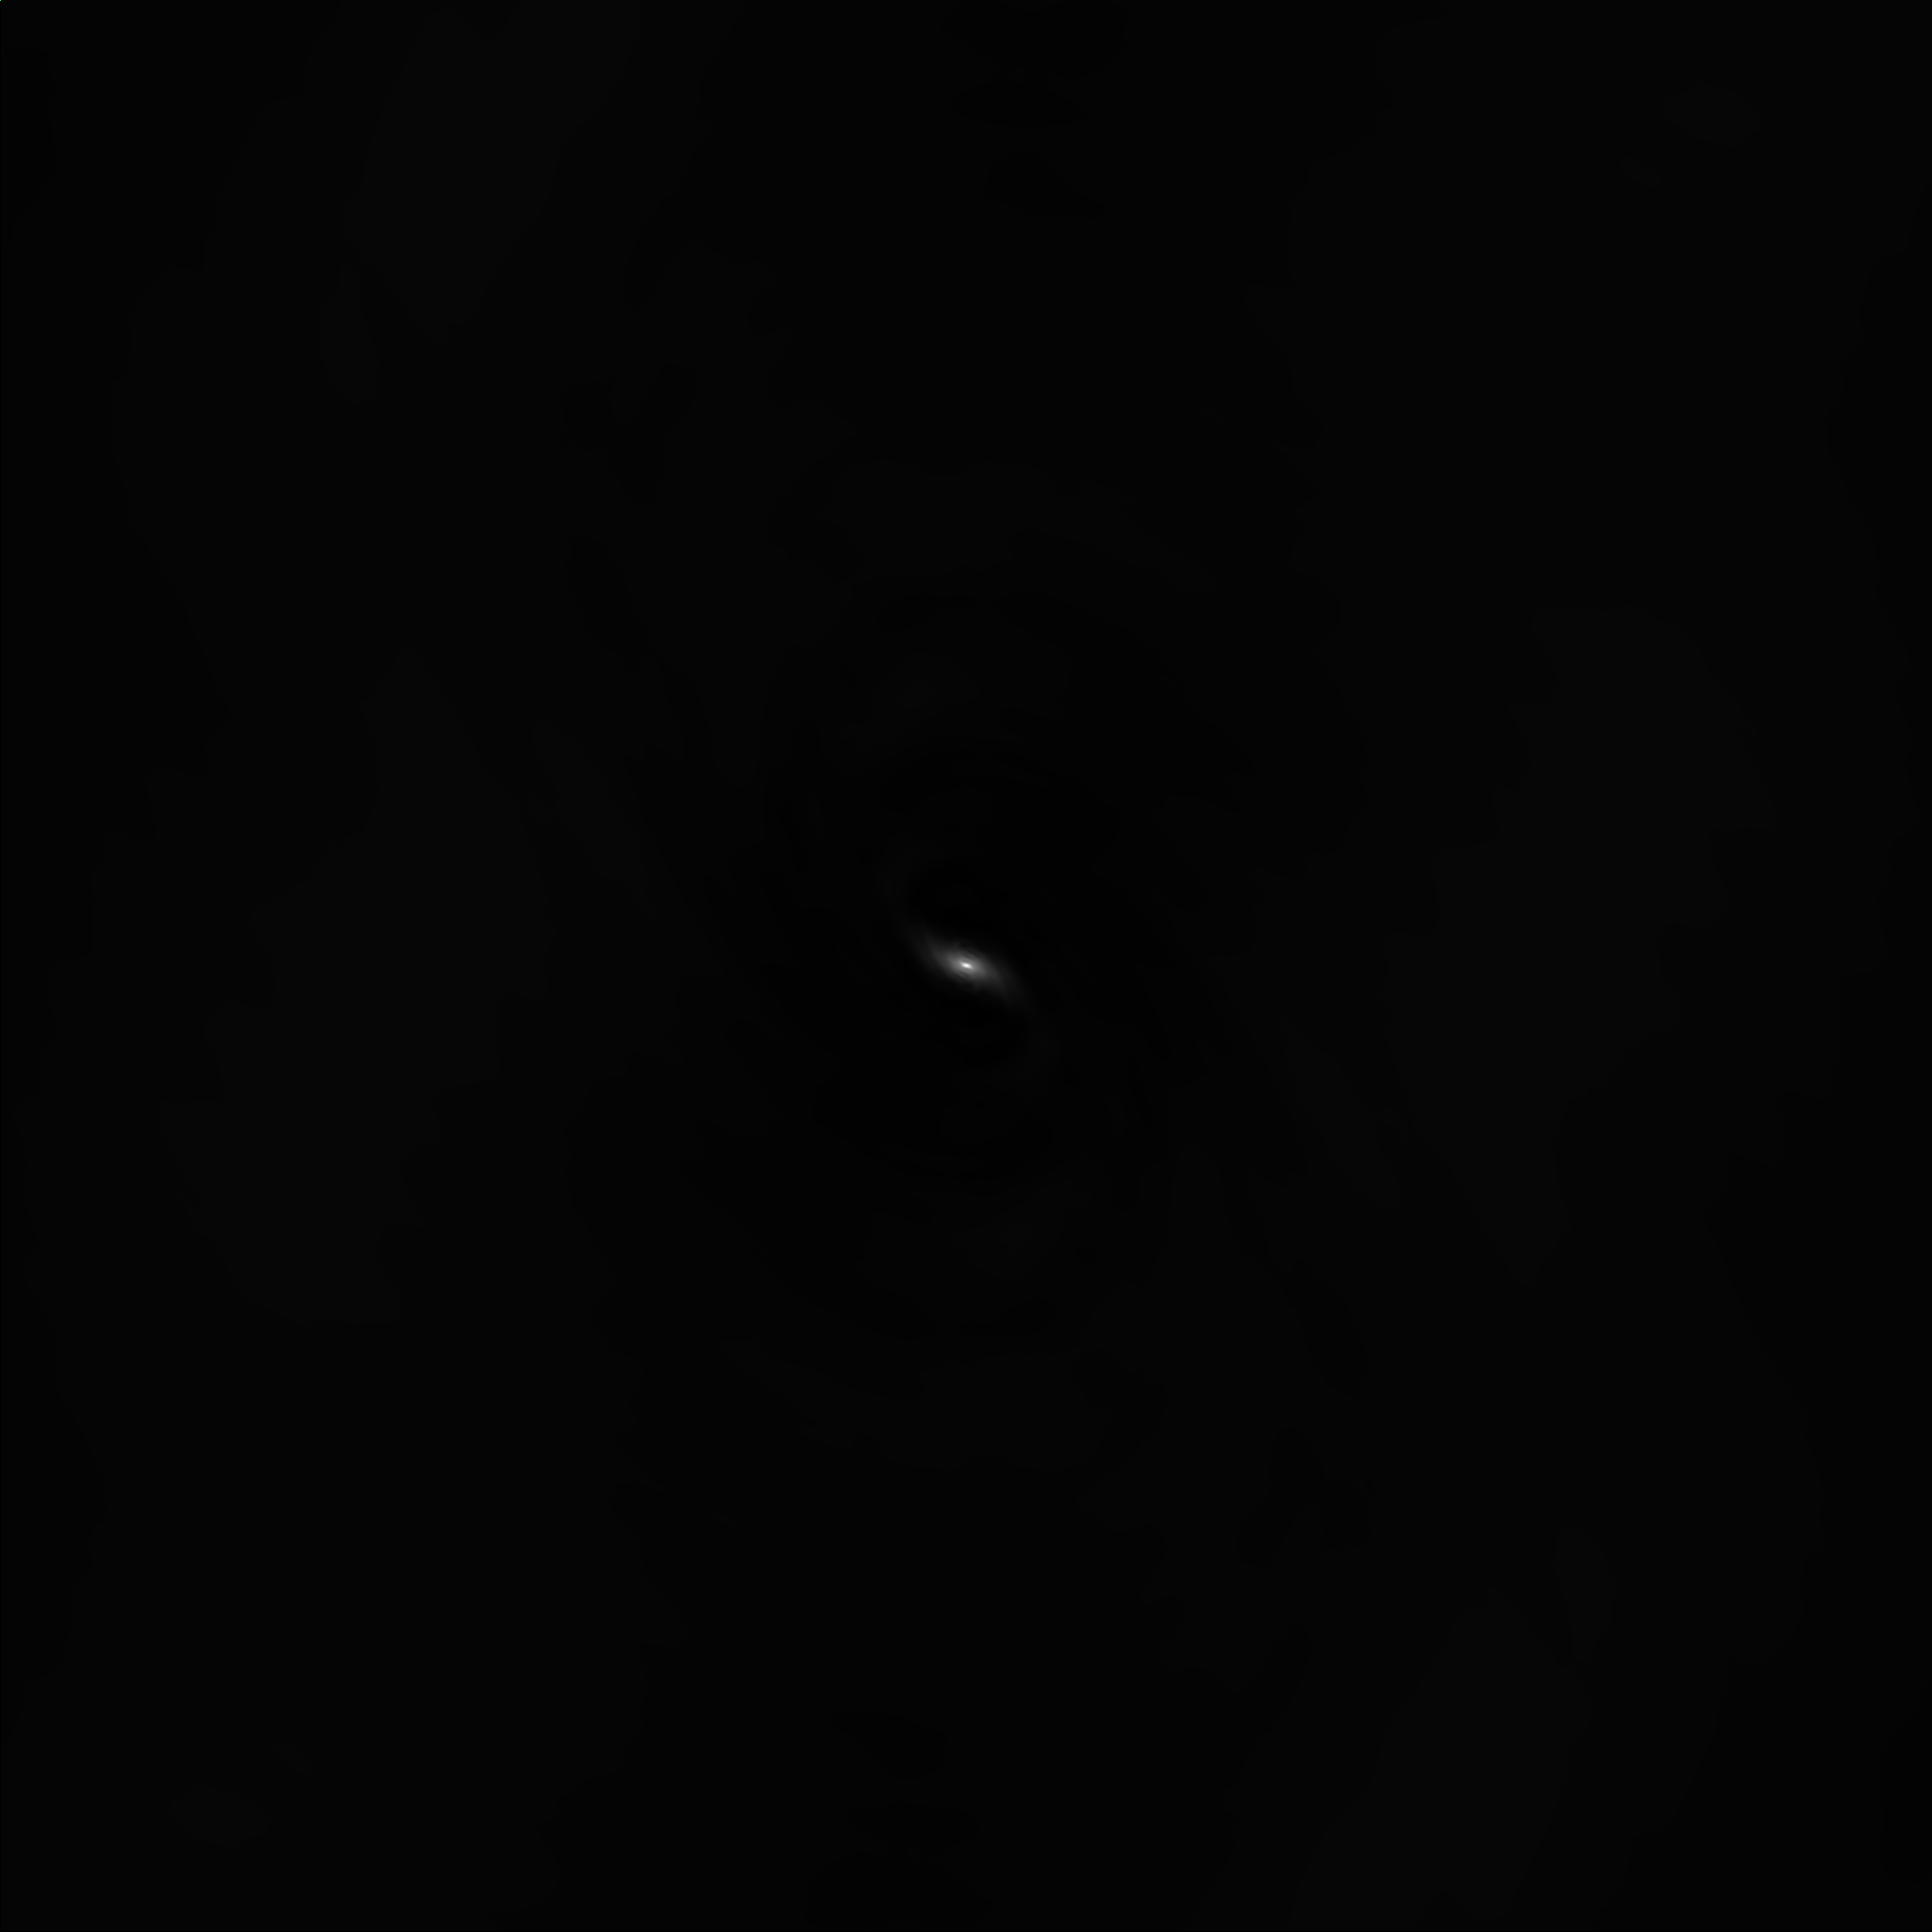
\includegraphics[width=\textwidth]{images/180min_single_7.png}
      \caption{7px full support}
    \end{subfigure}
    \begin{subfigure}[b]{0.45\textwidth}\centering
      
\includegraphics[width=\textwidth]{images/180min_single_15.png}
      \caption{15px full support}
    \end{subfigure}
    \begin{subfigure}[b]{0.45\textwidth}\centering
      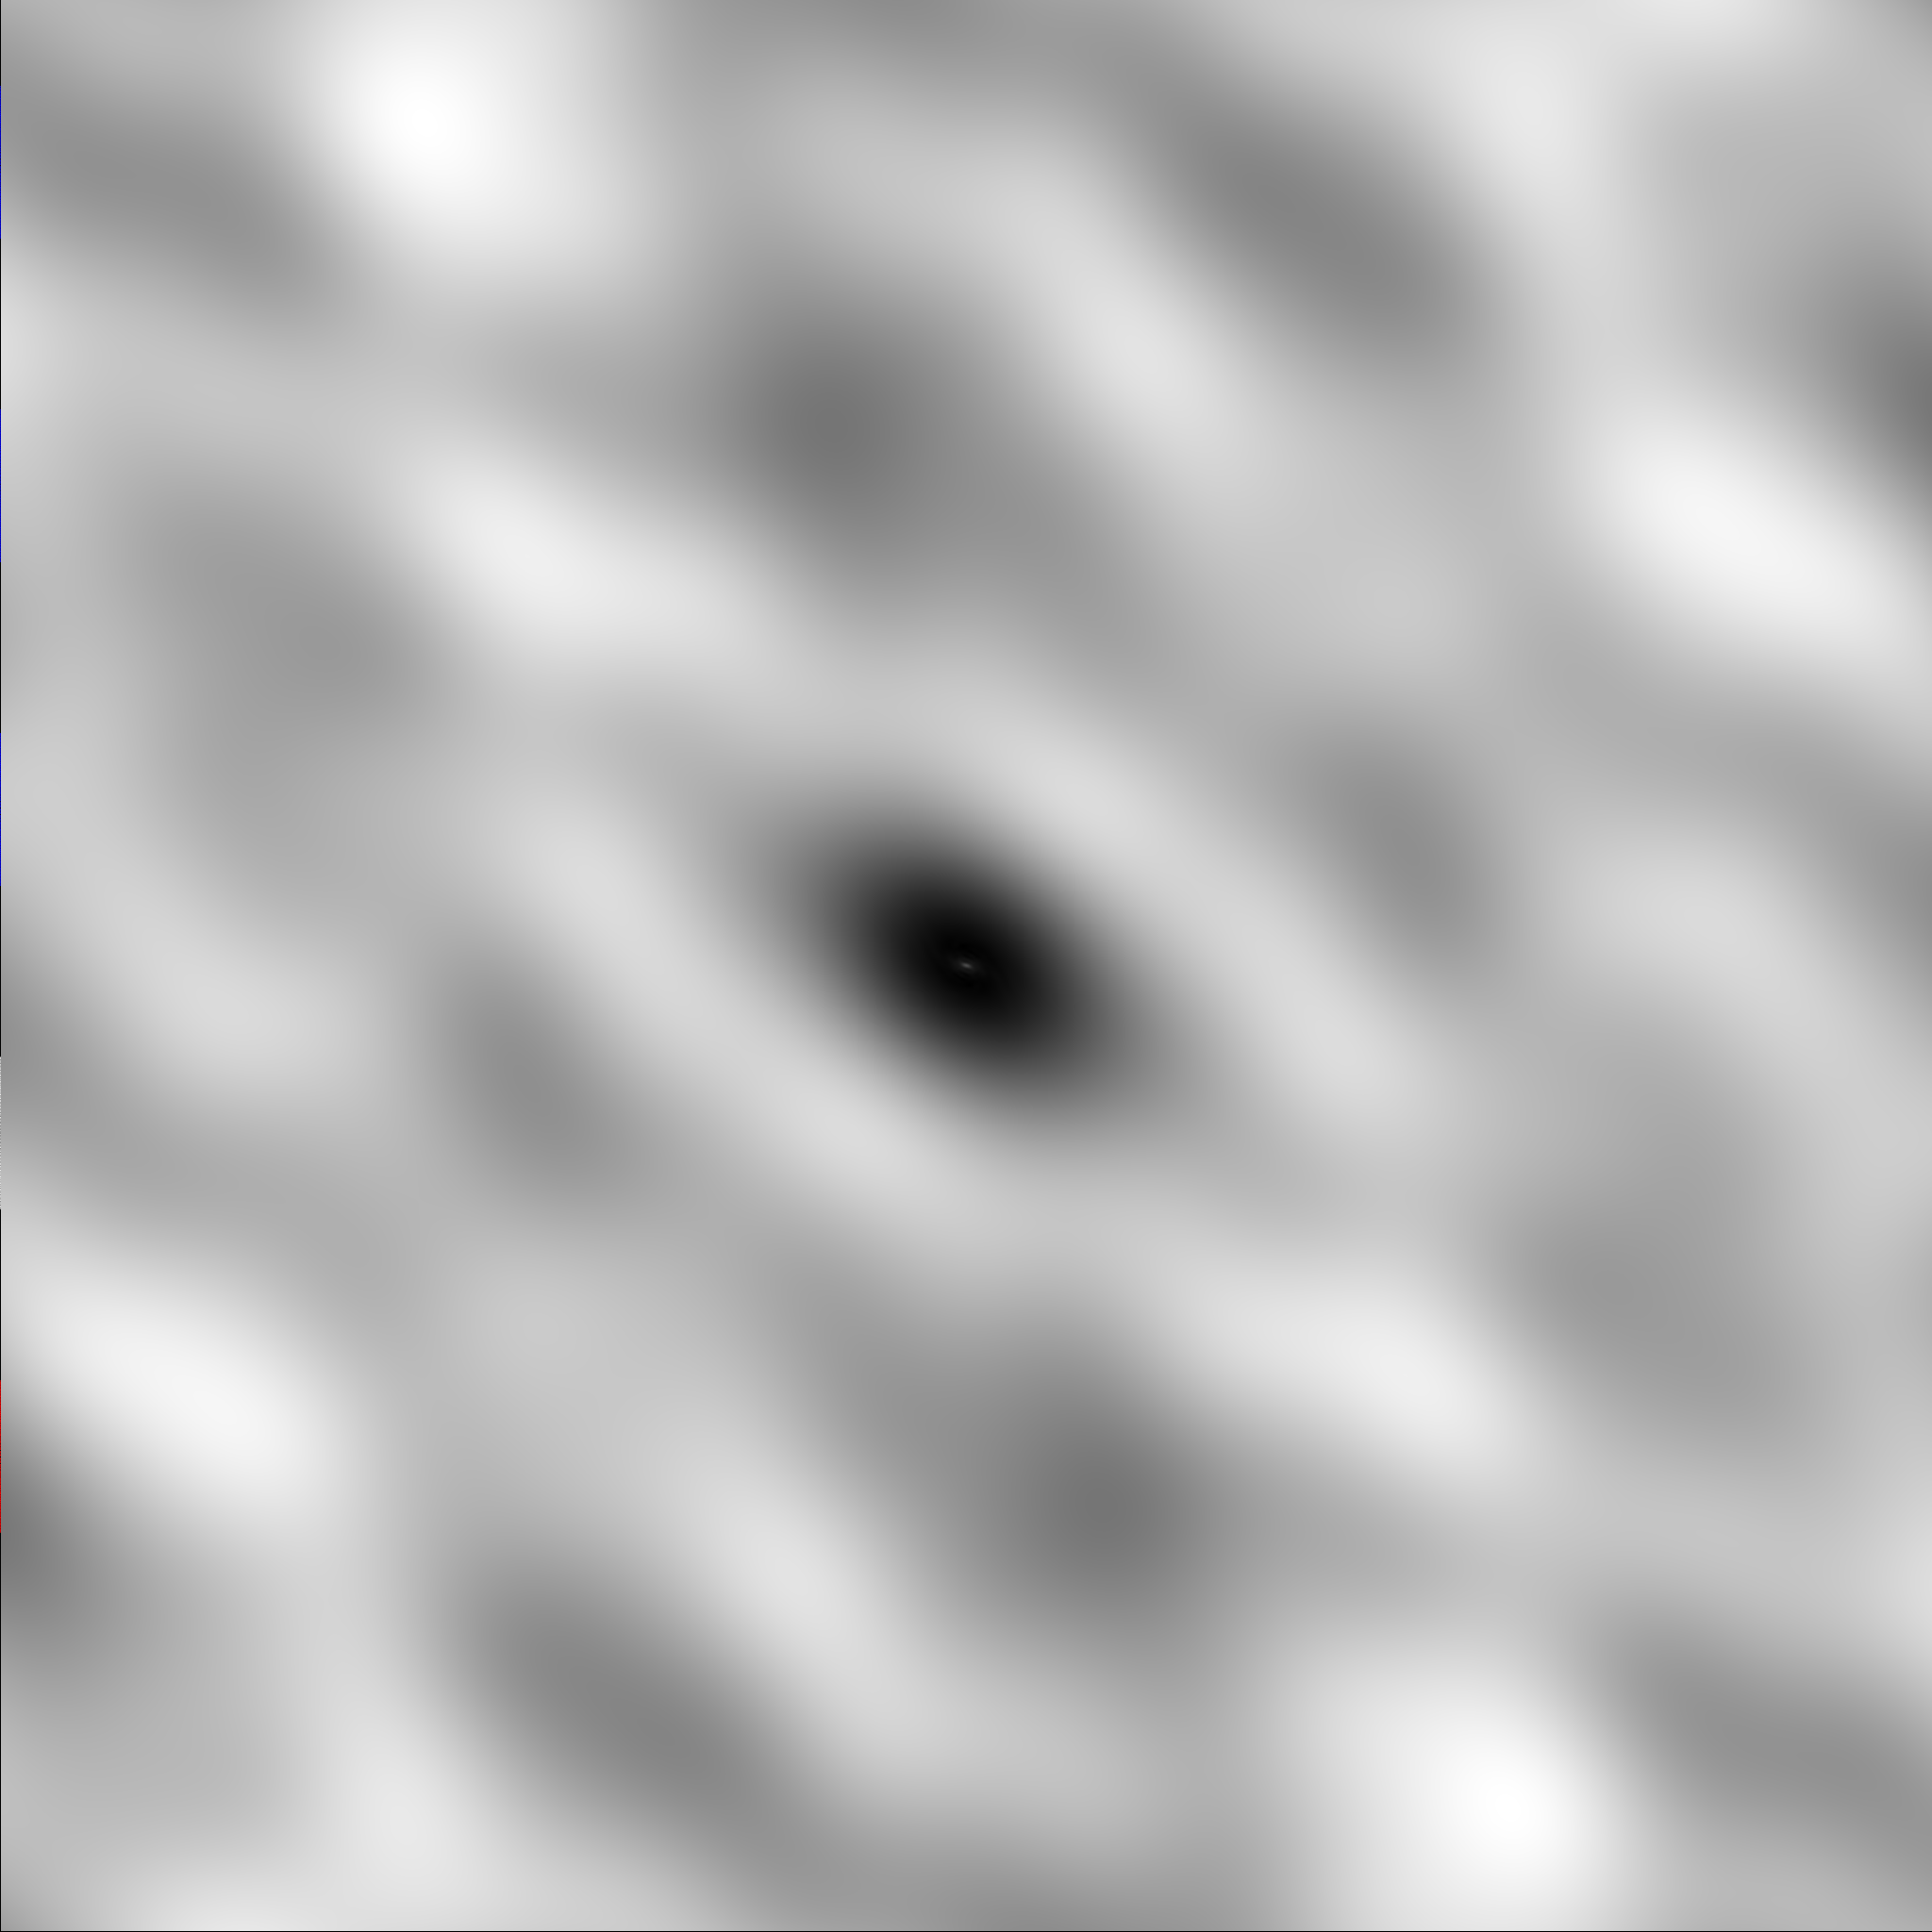
\includegraphics[width=\textwidth]{images/180min_single_23.png}
      \caption{23px full support}
    \end{subfigure}
    \caption[Precision error in simulated 3 hour MeerKAT observations]{This figure contains synthesized images when resampling 3 hour observations using filters with 7, 15 and 23 px full support sizes in single precision. We suspect 
    that there may be overflows on some of the grid cells because the measured brightness on the 23 px filter support image is negative. We eliminated the normalization counter as the cause of this problem since it is always computed in double precision
    and the double precision images remain accurate at a measured brightness of 1 Jy with a constant SNR.}
    \label{FIG_PREC_ERROR_IMAGES}
 \end{mdframed}
\end{figure}

\section{Profiling and implementation comments}
The NVIDIA Visual Profiler shows that the single precision gridding algorithm\footnote{Faceting a single correlation, with w-projection code disabled by means of templated 
traits and policies. These figures were obtained running on a GT960.} consists of just over 40\% integer arithmetic and only about 10\% single precision floating point arithmetic. These figures exclude the instructions wasted
on branch divergence. Our profiling also shows that the implementation is firmly bounded by memory latencies. Surprisingly this is not due to the global memory bandwidth 
(profiling shows that only about 10\% of the peak bandwidth is used), instead kernel register preasure is responsible for lowering the 
obtained occupancy (even for single correlation gridding). The combination of the low single precision floating point instruction usage 
and memory latencies results in a ~27\% utilization of available compute (Function Unit Utilization, as reported by the NVIDIA profiler). This 
also explains why the results indicate that double precision performance is not a third of single precision performance \footnote{The Kepler Architecture 
has 1 double precision arithmetic unit for every 3 single precision units}.

We suspect that the increased register usage of our algorithm and the resulting low compute utilization is one of the primary causes
of the large discrepency between the performance figures seen in John Romein's gridding benchmark\footnote{Code available at
\url{www.exaska.org/?q=Codes}} \cite{romein2012efficient} and our implementation. Our implementation is somewhat more general, and therefore 
algorithmically more complex than the benchmark implementation. Bullseye is able to handle common imaging use-cases, such as forming continuum 
image cubes, by dividing the available observation bandwidth (which may be spread out over multiple spectral windows) between grids for example, whereas 
this would require preprocessing the data and running Romein's implementation multiple times. We also do not precompute and 
store a set of uvw coordinates per channel because of the considerable memory requirements when dealing with larger databases, 
instead these are scaled by frequency on the fly. Some necessary memory accesses to visibility weights and flagging information, and 
the assocated branching that is common in imaging implementations are also missing from the benchmark.